\begin{lstlisting}
    p25 2
    p26 3(2)(3)
    p26 4(1)(3)
    \end{lstlisting}
\begin{figure}[H]
    \centering
    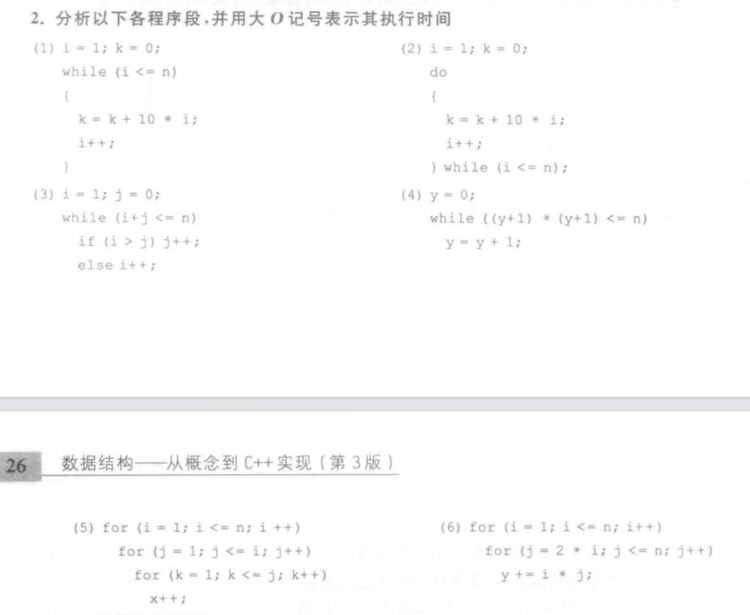
\includegraphics[width=\textwidth]{3-hw1-20250311.png}
    % \caption{}
    \label{}
\end{figure}

(1) $O(n)$
(2) $O (n)$
(3) $O(n)$
(4) $O(n^{1/2 })$
(5) $O(n^{3})$
(6) $O(n^{2})$

\begin{figure}[H]
    \centering
    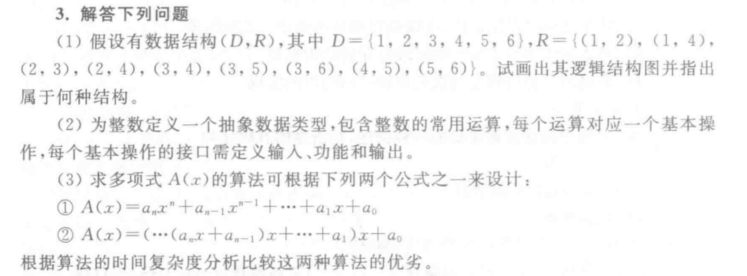
\includegraphics[width=\textwidth]{1-hw1-20250311.png}
    % \caption{}
    \label{}
\end{figure}

(2)

\begin{lstlisting}
    ADT integer
    
    DataModel
        integer: positive integer (1,2,3,...), negative integer (-1,-2,-3,...) and zero (0)
    
    Operation
        Plus
            输入:整数a和整数b
            功能:将整数a和整数b的值相加
            输出:相加后的结果a+b
        Minus
            输入:整数a和整数b
            功能:将整数a的值减去整数b的值
            输出:相减后的结果a-b
        Multiplicate
            输入:整数a和整数b
            功能:将整数a和整数b的值相乘
            输出:相乘后的结果a*b
        Divide
            输入:整数a和整数b
            功能:将整数a的值除以整数b的值
            输出:相除后的结果a/b
    \end{lstlisting}
(3)
第一种算法要进行 $1+2+\dots+n=\frac{n(n+1)}{2}$ 次乘法运算, $n$ 次加法运算。一共 $\frac{n^{2}}{2}+\frac{3n}{2}$ 次运算。
第二种算法要进行 $n$ 次乘法运算,$n$ 次加法运算。一共 $2n$ 次运算。
于是,第一种的时间复杂度为 $O(n^{2})$,第二种为 $O(n)$,所以第二种算法更优。

\begin{figure}[H]
    \centering
    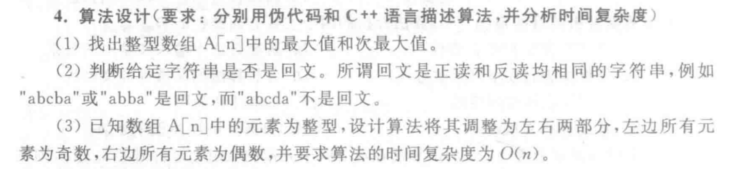
\includegraphics[width=\textwidth]{2-hw1-20250311.png}
    % \caption{}
    \label{}
\end{figure}

(1)
伪代码:

\begin{lstlisting}
    max1 = max(A[0], A[1]), max2 = min(A[0], A[1])
    for (i = 2; i < n; i++)
        if (A[i+1] > A[i])
            max2 = max1
            max1 = A[i+1]
    \end{lstlisting}
C++ 代码:

\begin{lstlisting}[language=C++]
    void Max_NextMax(int A[], int n, int &max1, int &max2) {
        if (n < 2) {
            // 处理数组元素不足两个的情况
            if (n == 1) {
                max1 = A[0];
                max2 = A[0]; // 或者设置为某个特定值表示没有次大元素
            }
            return;
        }
        // 初始化max1和max2
    
        max1 = std::max(A[0], A[1]);
        max2 = std::min(A[0], A[1]);
    
        // 遍历数组找出最大和次大元素
        for (int i = 2; i < n; i++) {
            if (A[i] > max1) {
                max2 = max1;
                max1 = A[i];
            } else if (A[i] > max2) {
                max2 = A[i];
            }
        }
    }
    \end{lstlisting}
一共进行了 $n-2$ 次运算,故时间复杂度为 $T(n)=O(n)$.

(3)
伪代码:

\begin{lstlisting}
    j = 0, k = 0
    for (i = 0; i < n; i++)
        if (i % 2 == 1)
            B[j++] = A[i]
        else
            C[k++] = A[i]
    for (i = 0; i < j; i++)
        A[i] = B[i]
    for (i = j; i < n; i++)
        A[i] = C[i-j]
    \end{lstlisting}
C++ 代码:

\begin{lstlisting}[language=C++]
    void SeparateOddEven(int A[], int n) {
        // 创建临时数组存储奇数和偶数
        int* B = new int[n]; // 存储奇数
        int* C = new int[n]; // 存储偶数
        int j = 0, k = 0;
    
        for (int i = 0; i < n; i++) {
            if (A[i] % 2 == 1) // 奇数放入B数组
                B[j++] = A[i];
            else // 偶数放入C数组
                C[k++] = A[i];
        }
        // 将奇数复制回原数组的左边
        for (int i = 0; i < j; i++)
            A[i] = B[i];
        // 将偶数复制回原数组的右边
        for (int i = j; i < n; i++)
            A[i] = C[i-j];
        // 释放临时数组
        delete[] B;
        delete[] C;
    }
    \end{lstlisting}
一共进行了 $2n$ 次赋值,时间复杂度为 $T(n)=O(n)$.
